% protocol.tex -- sources: PREREG-GATE-MUST-v3-2026-10-28.md (frozen at commit 164a18a5), SAP-GATE-2026-10-28.md (with
% Addenda 1 and 2), GATE-METHOD-SPEC-v2-2026-10-28.md. Precedence: SAP Addendum 2 > Addendum 1 > SAP > spec v2 > spec v1.
% Numbers in this file come from the preregistration documents (design values) or from runs/P2-PROBE-01/summary.json (pilot).
% No GATE outcome exists yet.

The protocol was fixed before any outcome of the main run existed.
It is recorded in a preregistration card, a statistical analysis plan with two addenda, and a method specification, all
pinned by commit and hash (Section~\ref{ssec:prereg}).
This section states what was run, with what, and how the results will be judged.
Parts of the method that the preregistered run does not exercise are named as such.

\subsection{Model, data and tokenisation}\label{ssec:data}
The model is UniDisc with 1.4B parameters~\cite{swerdlow2025unidisc}, used as released, with no training or finetuning here.
Images and captions come from the COCO val2017 split~\cite{lin2014coco}.
Images are tokenised at $512$~px with the VQ-16 tokenizer of LlamaGen~\cite{sun2024llamagen}, giving a $32\times32$ grid of
$m=1024$ image tokens drawn from 16\,384 codes.
Captions of 5 to 32 text tokens are used.
Instance annotations of val2017 are used to restrict wrong captions (Section~\ref{ssec:folds}).
Whether COCO val2017 images were in the training data of UniDisc or of the tokenizer is unknown to the authors and is a stated
limitation (Section~\ref{sec:discussion}).
The backbone runs in \texttt{bf16}; log-probabilities are an \fp{} log-softmax of the logits restricted to the scored modality.
The model is treated as time-independent, as in the released inference path, which calls the network without a noise-level input.

\subsection{Folds, negatives and tokeniser check}\label{ssec:folds}
% run: P2-GATE-FOLDS
Four disjoint sets of images are drawn by COCO image id with a fixed seed (20261029): calibration (300 items), headroom
(100), test (300, with an ordered extension to 500 used only if the sample-size rule of Section~\ref{ssec:headroom} asks
for it), and the 200 items of an earlier detection pilot, which serve as the detection set.
All new folds exclude the 494 image ids of the two pilots.
The fold file has SHA-256 \texttt{450edb54...f311} (full hash in the data statement).
The wrong caption $c^-$ of an item is a caption of another image, fixed once per item and shared by every arm and
corruption; where annotations exist, it comes from an image that shares no annotated COCO category with the true image.
Before any score is computed, the frozen caption token counts are compared with the counts of the runtime tokeniser.
An item whose real count falls outside 5 to 32 is excluded from every analysis, counted and not replaced; if more than
10\,\% of any fold fails the check the run stops and a fold-construction defect is reported.

\subsection{Corruptions}\label{ssec:corruptions}
Table~\ref{tab:corruptions} lists the corruptions.
Three are \emph{realistic}: they act on pixels before tokenisation and produce plausible codes.
Two are \emph{sanity} corruptions that replace tokens by uniform random codes; they are not in the primary family.
The corrupted-token label is $Z_j=\ind[\tilde v_j\neq v^\circ_j]$, relative to the tokenisation of the clean image.
Noise draws and the donor image and location of a splice derive from the item id, so one corruption realisation exists per image.

\begin{table}[t]
\centering
\caption{Corruptions. Realistic corruptions are walked in order by the headroom rule (Section~\ref{ssec:headroom}); the first
rung that passes is the operating point. Sanity corruptions have one setting.}
\label{tab:corruptions}
\small
\begin{tabular}{p{0.22\linewidth}p{0.2\linewidth}p{0.44\linewidth}}
\toprule
Corruption & Rungs & Definition \\
\midrule
JPEG (realistic) & quality 10, then 5 & JPEG compression of the 512-px pixels, then tokenisation \\
Gaussian noise (realistic) & $\sigma=0.10$, then $0.20$ & noise on pixels scaled to $[0,1]$, clipped and rounded to 8 bit, then tokenisation \\
Pixel splice (realistic) & $128\times128$, then $192\times192$ px & a region from a donor COCO image copied to a uniformly random location \\
Patch (sanity) & one $8\times8$ block & a block of the token grid replaced by uniform random codes \\
Swap (sanity) & 15\,\% of tokens & tokens replaced by uniform random codes \\
\bottomrule
\end{tabular}
\end{table}

\subsection{Headroom rule and sample size}\label{ssec:headroom}
A gate can restore verification only if corruption lowers it and removing the corrupted tokens recovers it.
Both are checked on the 100 headroom items, blind to the method: no gate flag is computed on those items.
The endpoint is the size-normalised evidence $d_R$ of Eq.~\eqref{eq:dz}.
For corruption $c$ and rung $r$ let $u_i=d^{\rm clean}_i-d^{\rm cor}_i$ and $v_i=d^{\rm chg}_i-d^{\rm cor}_i$, where
``chg'' is the changed-code gate that keeps exactly the tokens that did not change.
With $T_1$ and $T_2$ the paired $t$ statistics of $u$ and $v$ over the $n_v$ items that have all values, a rung passes if
$n_v\ge90$, $T_1\ge2.0$ and $T_2\ge2.0$.
The first passing rung of a corruption is its operating point; a corruption that passes neither rung has none, is not tested,
and keeps a $p$-value of one in the primary family.
If no corruption has an operating point, the downstream claim is withdrawn and the paper reports detection, calibration and the
clean control only.

The headroom items also fix the test-fold size.
Let $D_c$ be the number of headroom items whose paired correctness differs between the changed-code gate and no gate, and
$D^\ast=\max_c D_c$ over corruptions with an operating point.
Rule~R1 ($D^\ast\ge29$): test on the first 300 ids with the correctness endpoint.
Rule~R2 ($18\le D^\ast<29$): test on the first 500 ids.
Rule~R3 ($D^\ast<18$): test on the first 300 ids with the paired change of $d_R$ as the primary endpoint and correctness as a
secondary one.
The decision, $D_c$ and $D^\ast$ are written to a file that is committed before the first test item is scored.

\subsection{Arms and controls}\label{ssec:arms}
Table~\ref{tab:arms} lists the arms of the image-direction analysis.
All arms reuse the two caption-only passes per item (Table~\ref{tab:cost}).
The primary contrast is the marginalise arm (\emph{GATE-M}) against \emph{none}.
The controls separate three competing explanations: mask geometry (an equally shaped mask elsewhere), texture or encoder
instability (cheap non-generative detectors), and pixel denoising.

\begin{algorithm}[t]
\caption{\textsc{GeometryMatchedGate}: a random gate with the shape of the gate}\label{alg:geo}
\Input{gated set $G$ on the $32\times32$ grid; seed}
\Output{a random gate $G^{\rm geo}$ of the same size and shape at another place}
\Fn{\textsc{GeometryMatchedGate}$(G,\mathrm{seed})$}{
  draw $(d_x,d_y)$ uniformly from $\{0,\dots,31\}^2\setminus\{(0,0)\}$\;
  \Return $\{((x+d_x)\bmod32,\ (y+d_y)\bmod32):(x,y)\in G\}$ \Comment*[r]{torus shift}
}
\end{algorithm}

\begin{table}[t]
\centering
\caption{Arms of the image-direction analysis. $R$ is the set of image tokens kept in the sum of Eq.~\eqref{eq:delta}.}
\label{tab:arms}
\small
\begin{tabular}{p{0.25\linewidth}p{0.4\linewidth}p{0.23\linewidth}}
\toprule
Arm & Kept set $R$ & Role \\
\midrule
none & all 1024 tokens of the corrupted image & reference \\
GATE-M & tokens not flagged by the frozen gate (Algorithm~\ref{alg:gate_set}) & primary arm \\
geometry-matched random gate & complement of Algorithm~\ref{alg:geo} applied to GATE-M's mask, 3 seeds & mechanism control \\
scattered random gate & complement of equally many random tokens, 3 seeds & mechanism control \\
changed-code gate & tokens whose code did not change & upper reference for sanity corruptions only \\
plain-$B$ top-$k$ & complement of the $|G|$ tokens with the lowest $B_j$ & gate without calibration, equal size \\
$s_3$ top-$k$ & complement of the $|G|$ tokens with the largest $1-\max_y p_\theta$ & uncertainty-ranked gate, equal size \\
pixel denoise & none, on a denoised copy of the image (JPEG and noise) & defence comparator \\
GATE on clean images & as GATE-M on uncorrupted images & negative control \\
\bottomrule
\end{tabular}
\end{table}

\subsection{Detection baselines and comparators}\label{ssec:baselines}
Detection of changed codes is evaluated against four non-generative or uncalibrated rivals, all fixed in advance:
the \emph{patch texture} (pixel variance of the $16\times16$ patch of a token), the \emph{neighbour codebook distance}
(mean $L_2$ distance of the token's codebook vector to its eight neighbours), the \emph{code rarity} (negative log frequency of the
code among the calibration fold's clean codes), and the \emph{uncertainty score} $s_3$ above.
Both signs are admitted for each rival, which favours the rival (a sign oracle).
Plain-$B$ ($B_j$ without the null term) is the detector of Eq.~\eqref{eq:suspicion} without the null normalisation, and the score
$A_j-B_j$ is the cancellation control (expected near 0.5).
The three families of comparator that the related work names are handled as follows.
\emph{TbV-score (non-finetuned).} The observed-position probability of Trust but Verify~\cite{jhingran2026trustverify}
computed from the raw backbone logits of the unmodified model with the caption masked, never from the released
output layer, which writes a probability of one at every unmasked position.
It reproduces the score of that paper but not its method, which needs a finetune that is outside this study.
It is reported threshold-free, and it is marked not applicable if the raw logits turn out to be degenerate.
\emph{UniDisc repair recipe}~\cite{swerdlow2025unidisc}: random mask of equal size, $n$ re-infills, best of $n$ by the model's
own likelihood, at matched network calls.
This comparator belongs to the re-infill tier, which is not frozen; if it is run, an addendum is written before its first item,
and otherwise the paper says that it was not run.
\emph{Pixel denoiser}: OpenCV non-local-means denoising for colour images, one setting for all corruptions, with strength
$h=h_{\rm color}=25.5$ grey levels (matched to the noise level $0.10\times255$) and windows of 7 and 21 pixels.
% run: P2-GATE-CPU/denoise_check
On 20 images this setting raises the PSNR of the noisy image at $\sigma=0.10$ from 20.41 to 25.75~dB, and lowers that of JPEG
quality~10 from 26.82 to 25.13~dB.
The denoiser is therefore not neutral on JPEG: against it GATE-M is compared with an aggressive denoiser that harms the image,
and the JPEG row is worded accordingly.
Token-Critic~\cite{lezama2022tokencritic}, CO2Jump~\cite{le2026co2jump} and FreeCorrection~\cite{ouyang2026freecorrection} are
discussed but not run: they need a trained critic, are sampler-level methods for generation, or have code that is not
runnable at the pinned commit.

\subsection{Endpoints and tests}\label{ssec:tests}
\paragraph{Primary family.}
For each of JPEG, noise and splice, at the operating point from the headroom rule, the endpoint is the paired correctness
$Y$ of Eq.~\eqref{eq:delta} under GATE-M against none.
The test is the exact two-sided McNemar test~\cite{mcnemar1947} on the discordant items: with $b$ items right under GATE-M and
wrong under none, $c$ items the reverse, and $n_d=b+c$,
\begin{equation}
p=\min\Big\{1,\ 2\,\PP\big(\mathrm{Bin}(n_d,\tfrac12)\le\min(b,c)\big)\Big\}.
\label{eq:mcnemar}
\end{equation}
The family has exactly three hypotheses at all times, with Holm step-down~\cite{holm1979sequentially} at familywise level 0.05:
a corruption without an operating point stays in the family with $p=1$.
The headline claim is supported only if at least one hypothesis is rejected after Holm with $b>c$; a rejection with $c>b$ is
reported as ``GATE-M worse than none''.
With every test the paper reports $b$, $c$, $n_d$, $n$, both accuracies, the net difference $(b-c)/n$ with paired bootstrap
intervals (10\,000 resamples) at 95\,\% and at 98.33\,\%, and the Clopper--Pearson interval~\cite{clopper1934} of $b/n_d$.
The design minimum detectable net gain at $n=300$ is 0.053 unadjusted and 0.060 at the first Holm step, under an assumed
discordance of 10\,\% (assumed, not observed).

\paragraph{Secondary families (each with its own Holm correction, none able to rescue a failed primary test).}
Table~\ref{tab:families} lists them.
Everything else is exploratory, reported with intervals and without $p$-values that enter a claim.

\begin{table}[t]
\centering
\caption{Secondary confirmatory families. $m$: number of hypotheses in the family's Holm correction.}
\label{tab:families}
\small
\begin{tabular}{p{0.2\linewidth}p{0.6\linewidth}p{0.05\linewidth}}
\toprule
Family & Contrast and test & $m$ \\
\midrule
Mechanism & GATE-M versus the geometry-matched random gate (seed 1), exact McNemar; tested only for corruptions rejected in the primary family & 3 \\
Evidence ratio & paired change of $d_R$, GATE-M minus none, Wilcoxon signed rank & 3 \\
Denoising & GATE-M versus the pixel denoiser, exact McNemar; JPEG and noise only & 2 \\
Detection & per-item AUROC of $q$ minus that of the best cheap rival on the 200 detection items, JPEG quality 10 and noise 0.10; paired bootstrap over items & 2 \\
Out-of-sample detection & the same contrast with the rival frozen after the detection run, on the test items at their operating points & 2 \\
Clean control & GATE-M versus none on clean test images, exact McNemar & 1 \\
\bottomrule
\end{tabular}
\end{table}

\paragraph{Calibration diagnostics.}
On the clean test items, the realised false-alarm proportion $\hat F=n^{-1}\sum_i L_i(\hat\tau)$ is reported for
$\alpha\in\{0.01,0.05,0.10\}$, with $\alpha=0.05$ primary and the others unselected sensitivities.
A violation is flagged when $Z_{\rm cal}=(\hat F-\alpha)/\big(\hat\sigma_L\sqrt{1/n_{\rm cal}+1/n_{\rm test}}\big)$ exceeds 2.13 at any
level, where $\hat\sigma_L$ is the pooled item-level standard deviation of $L_i$.
A pass means ``no evidence of violation'' and is never worded as validation.
Reported with equal prominence: the precision among flagged tokens per corruption, the false-alarm proportion on the clean tokens
of corrupted items, and the spatial map of clean false alarms.
For $\alpha=0.05$ on an $8\times8$ patch image, about 48 false flags are expected against at most 64 true ones, so precision is at
most 0.57 even for a perfect detector.

\paragraph{Pipeline checks and positive controls.}
For the sanity corruptions, the lower bound of the 95\,\% interval of the per-item AUROC of $q$ and of plain-$B$ against the
changed-code labels must exceed 0.5; a result at chance is a pipeline defect, not a scientific result, and triggers an audit without
any change of rule.
The clean no-gate accuracy of the image direction is reported with a Wilson interval against the pilot value of
Section~\ref{ssec:pilot} as a descriptive pipeline check; it is not a validation and tests nothing.
A coherence test measures, on 100 clean calibration items, whether the denoiser's joint likelihood of two image tokens is
independent of the order in which they are revealed.
Its pre-stated reading is ``coherent within numerical noise'' if the median absolute gap lies within the 95th percentile of the
gap between repeats of the same computation, and ``incoherent at the evidence scale'' if it exceeds the clean mean per-token
paired evidence; in the second case Eq.~\eqref{eq:marginalise} and the marginalise--impute comparison are reported as not applicable
at the scale that matters.

\paragraph{Reading of results.}
The outcome is labelled \emph{positive} if at least one primary hypothesis is rejected after Holm with $b>c$, which supports only
``GATE-M improves image-direction verification over no gate on that corruption''; attribution to detection needs the mechanism
family.
It is \emph{negative} if no primary hypothesis is rejected and, for every corruption with an operating point, the 90\,\% paired
bootstrap interval of the net accuracy difference lies inside $(-0.05,+0.05)$ with at least 240 completed items.
It is \emph{inconclusive} otherwise.
A null result is worded ``no improvement was detected; the data are compatible with a net accuracy change between $L$ and $U$'', and
never ``GATE-M has no effect''.
Under rule~R3 the primary endpoint is the evidence ratio, the label negative is not available, and the positive sentence says that
GATE-M increased the evidence ratio and nothing about verification accuracy, with the caveat that removing heavy-tailed tokens can
raise a ratio for any reason.
Rules that stop the claim are fixed in advance: no corruption with an operating point, detection by $q$ not better than the best
rival on both JPEG and noise, no primary rejection, a $Z_{\rm cal}$ above 2.13, and more than 5\,\% empty or non-finite
evidence in an arm.

\subsection{Two-way fusion and the text direction}\label{ssec:fusionprotocol}
Two-way fusion is analysed only if the best single direction has a clean test accuracy below 0.95.
Otherwise the paper states that the fusion gain cannot be tested at that ceiling.
The text-direction conditioning arms (none, GATE-M with the flagged image tokens masked, geometry-matched, changed-code) run for the
three realistic corruptions and are exploratory.
Caption corruption, re-infilling and a hard-negative set are not part of the preregistered main run.
The title, abstract and highlights therefore make no claim about fusion, marginalisation versus imputation, re-infilling or
caption corruption, and the paper states that these were not tested unless an addendum adds them before the first item of the run
concerned.

\subsection{Exploratory feasibility result}\label{ssec:pilot}
% run: P2-PROBE-01
A pilot on 300 clean COCO images, run before the protocol was fixed, shows the pair-level signal on which the endpoint rests.
For each image the true caption was compared with a caption drawn from a different image, and accuracy is the share of images for which
the true caption scores higher (chance 0.5; bootstrap intervals over images, 10\,000 resamples).
With $K=8$ complementary masks and the other modality visible, the text direction reaches 0.730 (95\,\% interval 0.680 to 0.777) and the
image direction 0.783 (0.737 to 0.830).
A caption-only control, with the whole image masked, stays at chance, 0.497 (0.440 to 0.553), so the text-direction value is not explained
by caption fluency.
Variants chosen after seeing these results, with all tokens of the scored modality masked in one pass and the image-masked null
subtracted, reach 0.990 (0.977 to 1.000) in the text direction and 0.843 (0.803 to 0.883) in the image direction, 253 of 300 images
(Figure~\ref{fig:probe1}).
The image-direction accuracy of 0.843 is the headroom that makes it, and not the text direction, the primary endpoint: the text
direction sits near a ceiling at which restoration cannot be shown.
The mean paired margin of that image-direction statistic is 0.18 nats per token.
This is a single run with one mismatch draw, on clean images, with the full-mask variants selected post hoc; it is exploratory and
carries no inference beyond the intervals shown.

\begin{figure}[t]
\centering
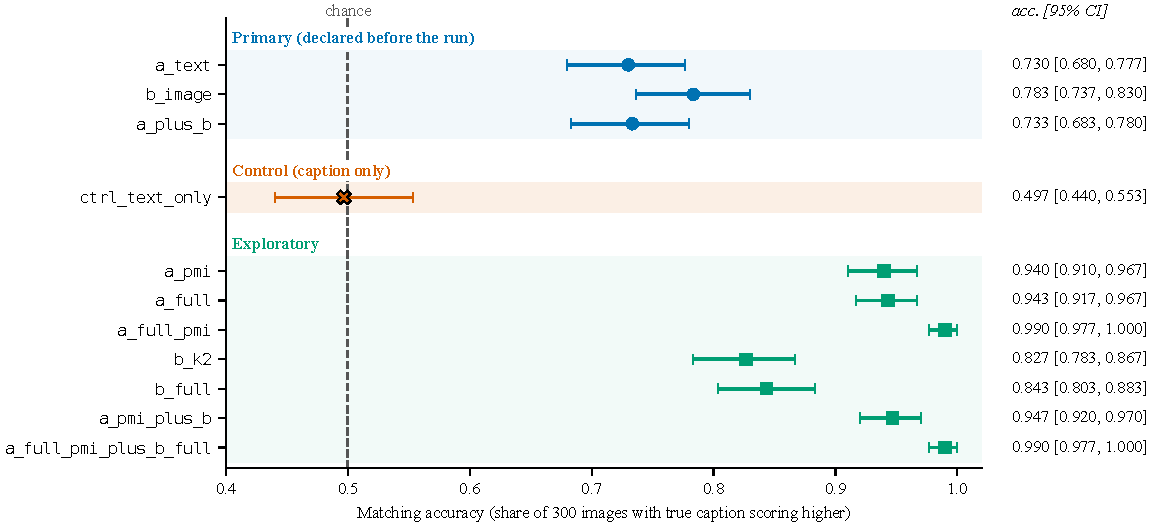
\includegraphics[width=0.92\linewidth]{figures/F1_probe1_accuracy.pdf}
\caption{Matching accuracy of UniDisc 1.4B on true versus mismatched COCO captions (exploratory feasibility result, 300 images).
Markers show the share of images for which the true caption scores higher (chance 0.5, dashed); bars are 95\,\% bootstrap intervals
over images (10\,000 resamples). Blue: primary scores, text direction a\_text and image direction b\_image with $K=8$ complementary
masks, and their sum. Orange: caption-only control, which stays at chance. Green: variants chosen after the primary results (image-masked
null subtracted, single full-mask pass, $K=2$, sums). One run, one mismatch draw; the intervals do not cover variation across draws or
models.}
\label{fig:probe1}
\end{figure}

\subsection{Hardware, runtime and missing items}\label{ssec:hardware}
% run: P2-PROBE-01
All runs use one laptop GPU (NVIDIA RTX 5070 Ti Laptop, 12~GB) with 31~GB of system memory and no other hardware.
In the pilot, one item cost 58 network passes, the median item time was 7.0~s, and the peak GPU memory was 8.2~GB, which is why
passes are batched four rows at a time.
Runs go in short checkpointed chunks under a guard that stops on memory, temperature and power-source events and is resumable;
an abort ends the stage and is not retried until reviewed.
An earlier detection pilot stopped after 20 complete items when the GPU session failed.
% run: P2-PROBE-02
Missing items are handled by a fixed rule: complete cases per analysis, no replacements and no reordering, so that a crash leaves a
prefix of the item list; if the completed base fold has fewer than 240 items, the paper says that the fold is under 80\,\% complete,
prints the minimum detectable effect at the achieved $n$, and does not read ``not rejected'' as evidence against GATE-M.
No analysis that computes $Y$, $b$, $c$, $p$ or a difference of $d_R$ is run on test data before the planned fold is complete.
Mask-seed and corruption-seed variance are not in the intervals, which is a stated limitation.

\subsection{Preregistration, pins and disclosed deviations}\label{ssec:prereg}
The code, the tests, the fold file and the analysis plan are pinned: the code at commit \texttt{164a18a5}, the analysis plan by SHA-256
(\texttt{b4e0bf57...6c47}), and the denoiser check, crash diagnosis and audit files by hash in the repository.
Changes after the pin are logged as amendments; none is made inside a stage.
One analysis preceded the analysis plan and is disclosed.
% run: P2-GATE-CPU/m1_fallback
The first 21 items of the detection set were analysed on CPU before the plan's second addendum, without the gate statistic $q$ (which needs a
GPU pass).
In that exploratory look the mean per-item AUROC against changed-code labels of plain-$B$ was 0.54 on JPEG quality 10 and 0.51 on noise
0.10, while pixel variance with its sign flipped scored 0.76 and 0.77.
The sign of the pixel-variance rival therefore cannot be claimed to be fixed blind, which is why both signs of every rival are admitted
and the rival is chosen on the data.
Any change to the score, $K$, $\alpha$, folds, rungs, arms, family or rival rule that was made after that look and is not a new version of
the preregistration is listed in the change log of the preregistration card and disclosed here.
\todo{AUTHOR: final list of amendments and the date of the first M2 outcome; confirm the status of the open decisions on guard
thresholds, the JPEG denoiser setting and the fallback before the run.}
